%%%%%%%%%%%%%%%%%%%%%%%%%%%%%%%%%%%%%%%%%%%%%%%%%%%%%%%%%%%%%%%%%%%%%%%%%%%%%%%%%%%%%%%%%%%%%%%%%%%%%%%%%%%%%%%%%
%% Kapitel 2 - Stand der Forschung und Technik %%%%%%%%%%%%%%%%%%%%%%%%%%%%%%%%%%%%%%%%%%%%%%%%%%%%%%%%%%%%%%%%%%
%%%%%%%%%%%%%%%%%%%%%%%%%%%%%%%%%%%%%%%%%%%%%%%%%%%%%%%%%%%%%%%%%%%%%%%%%%%%%%%%%%%%%%%%%%%%%%%%%%%%%%%%%%%%%%%%%
\chapter{Stand der Forschung und Technik} \label{chap:stand}

Dieses Kapitel stellt die für diese Arbeit erforderlichen technischen und methodischen Grundlagen bereit. Zunächst werde in Abschnitt~\ref{sec:zuv} zentrale Begriffe und Konzepte der Zuverlässigkeitstechnik sowie das grundlegende statistische Verfahren zur Lebensdauer-Datenanalyse in Kombination mit Versuchsplänen erläutert.
Darauf aufbauend folgen in Abschnitt~\ref{sec:doe} die Einführung und die Einordnung von \acs{DoE} für Lebensdaueruntersuchungen sowie der multivariaten Lebensdauermodellierung aus dem Stand der Technik und der Wissenschaft, die beide für die Entwicklung effizienter Lebensdauerversuchspläne maßgeblich sind.
Im Kontext der Lebensdauererprobung umfasst dies insbesondere typische, statistische Versuchspläne sowie Metriken und Indikatoren zur allgemeinen Bewertung der Versuchspläne.

\section{Zuverlässigkeitstechnik und Wahrscheinlichkeitstheorie} \label{sec:zuv}
Die Zuverlässigkeitstechnik befasst sich mit der probabilistischen Beschreibung der Lebensdauer technischer Produkte und Systeme sowie der strategischen und statistischen Planung von Lebensdauertests.
Ziel ist die statistische Modellierung des Ausfallverhaltens unter Berücksichtigung der Funktionalität des Produkts bei relevanten Randbedingungen.
Eine zentrale Aufgabe besteht somit in der statistischen Charakterisierung des Ausfallbegriffs mithilfe deskriptiver Statistik sowie in der Parametrisierung geeigneter Verteilungen zur Abbildung des Lebensdauerverhaltens.
Die Modellierung kann - abhängig von den Randbedingungen - auf Basis \textit{einer einzelnen} Belastungsgröße oder \textit{mehrerer} Beanspruchungsparameter erfolgen, die gemeinsam den Produktausfall determinieren.
Ein grundlegendes Verständnis des Umgangs mit zufallsverteilten Lebensdauerereignissen ist daher eine elementare Voraussetzung für die statistische Versuchsplanung im Rahmen der Zuverlässigkeitstechnik.
Weiterführende Konzepte und vertiefte methodische Ansätze zur Zuverlässigkeitstechnik sowie zur statistischen Testplanung sind allen voran in der Standardliteratur von \textcite{Bertsche.2022} dargelegt, an deren Vorgehensweise sich die nachfolgenden Ausführungen orientieren.

\subsection{Begriffe und Definitionen} \label{subsec:begriffezuv}
Der \textbf{Ausfall} eines technischen Produkts bezeichnet den Zeitpunkt innerhalb seiner Lebensdauer, zu dem die geforderte Funktionalität unter definierten Umgebungs- und Randbedingungen nicht mehr erfüllt ist - also das Lebensdauerende - engl. \textbf{\ac{EoL}}.
Als \textbf{Belastung} werden die von außen auf ein Produkt einwirkenden Einflussparameter - Kräfte und Momente im mechanischen Kontext - bezeichnet.
\textit{Einzelne} oder zeitgleich \textit{mehrere} Einflussparameter induzieren infolge der Produktgestalt daraus \textbf{Beanspruchungen}: innere Kräfte, Momente und lokale Spannungen.
Belastung und Beanspruchung sind die maßgeblichen Faktoren, welche die Lebensdauer determinieren.
Die \textbf{Ausfallzeit}, welche diese Zustandsänderung zeitlich definiert, wird im Allgemeinen als kontinuierliche Zufallsvariable $\sym{tau}>0$ aufgefasst.
So ergibt sich die Wahrscheinlichkeit, dass ein Produkt im Zeitraum bis $\sym{t}$ einen Funktionsverlust erleidet, zu
\begin{equation} \label{eq:probdef}
    \sym{F}(\sym{t})=\sym{Pr}(\sym{tau}\leq \sym{t}) = \int_{0}^{\sym{t}} \sym{f}(\sym{t}) \,d\sym{t}.
\end{equation}
Diese Funktion beschreibt die \textbf{Ausfallwahrscheinlichkeit}.
Sie definiert damit die Verteilungsfunktion - engl. \textbf{\ac{cdf}} - für stochastische \ac{EoL}-Events, während die \textbf{Zuverlässigkeit}
\begin{equation} \label{eq:reldef}
    \sym{R}(\sym{t})=\sym{Pr}(\sym{tau} > \sym{t}) = 1 - \sym{F}(\sym{t}) = \int_{\sym{t}}^{\infty} \sym{f}(\sym{t}) \,d\sym{t} , \quad \sym{t} \geq 0.
\end{equation}
komplementär diejenige Wahrscheinlichkeit $\sym{R}(\sym{t}): \sym{RR}_{\geq 0} \rightarrow [0,1] \subset \sym{RR}$ quantifiziert, zu der das nicht reparierbare Produkt die realisierte Zeit $\sym{t}$ überlebt: also frei von Funktionsverlust bleibt und funktionsfähig ist \cite{Bertsche.2022,Birolini.2017,Meeker.2022}.
Damit ist die Zuverlässigkeit mathematisch als reellwertige, monoton fallende und stetige Funktion definiert.
Gleichwohl ist $\sym{R}(\sym{t})$ keine universelle Eigenschaft, sondern vielmehr eine Funktion der Betriebsbedingungen .
Diese Bedingungen umfassen unter anderem eine oder mehrere Belastungsarten und deren Niveaus, Nutzungsverhalten sowie
spezifische Betriebsprofile. Mechanische, elektrische und thermische Belastungen treten dabei am häufigsten auf \cite{Yang.2007}.
Die \textbf{Wahrscheinlichkeitsdichtefunktion} - engl. \textbf{\ac{pdf}} - $\sym{f}(\sym{t})$ der Ausfallzeit beschreibt, wie sich die Wahrscheinlichkeiten der Ausfälle über der Zeit verteilen.
Sie folgt somit der Ableitung der \ac{cdf}:
\begin{equation} \label{eq:pdfdef}
    \sym{f}(\sym{t}) = \frac{d}{d\sym{t}}\sym{F}(\sym{t}) = \frac{d}{d\sym{t}}\sym{Pr}(\sym{tau} \leq \sym{t}), \quad \sym{t} \geq 0.
\end{equation}
Damit repräsentiert $\sym{f}(\sym{t})$ die Ausfallintensität pro Zeiteinheit und ist proportional zur lokalen Änderungsrate der Ausfallwahrscheinlichkeit.
Als vierte fundamentale Größe der Zuverlässigkeitsanalyse wird außerdem die \textbf{Ausfallrate} (auch Hazard-Funktion) $\sym{lambda}(\sym{t})$ eingeführt.
Sie quantifiziert das momentane Ausfallrisiko eines Produkts zum Zeitpunkt $\sym{t}$, bedingt dadurch, dass es bis zu diesem Zeitpunkt überlebt hat ($\sym{R}(\sym{t}) > 0$).
Mathematisch ist sie als das Verhältnis der \ac{pdf} zur Zuverlässigkeitsfunktion $\sym{R}(\sym{t})$ definiert:
\begin{equation} \label{eq:hazarddef}
    \sym{lambda}(\sym{t}) = \lim_{\Delta \sym{t} \to 0} \frac{\sym{Pr}(\sym{t} < \sym{tau} \leq \sym{t} + \Delta \sym{t} | \sym{tau} > \sym{t})}{\Delta \sym{t}} = \frac{1}{\sym{R}(\sym{t})} \left[ - \frac{d\sym{R}(\sym{t})}{d\sym{t}} \right] = \frac{\sym{f}(\sym{t})}{\sym{R}(\sym{t})} .
\end{equation}
Die Ausfallrate $\sym{lambda}(\sym{t})$ ist von zentraler Bedeutung, da ihr zeitlicher Verlauf (z.B. konstant, steigend, fallend) direkte Rückschlüsse auf zugrundeliegende Ausfallmechanismen wie Frühausfälle, Zufallsausfälle oder Verschleiß (vgl. "Badewannenkurve") zulässt \cite{Bertsche.2022,Yang.2007,Rigdon.2022}.

\subsection{Deskriptive Statistik für Lebensdauerdaten} \label{subsec:stat}
Die im vorherigen Abschnitt definierten Funktionen $\sym{F}(\sym{t})$, $\sym{R}(\sym{t})$, $\sym{f}(\sym{t})$ und $\sym{lambda}(\sym{t})$ beschreiben das stochastische Ausfallverhalten eines Produktes auf einer theoretischen Populationsebene.
Für die praktische Anwendung im Engineering müssen diese Funktionen, respektive die Parameter der ihnen zugrundeliegenden Verteilungsmodelle, auf Basis von empirisch ermittelten Lebensdauerdaten jedoch approximiert werden.

Die deskriptive Statistik stellt die notwendigen Methoden zur initialen Charakterisierung, Quantifizierung und Aufbereitung dieser Stichprobendaten bereit.
Zur Beschreibung der Lebensdauerverteilungen sind \textbf{Lageparameter} und \textbf{Streuungsmaße} notwendig, die zunächst theoretisch (für die Grundgesamtheit) definiert und anschließend aus der Stichprobe berechnet werden.

Der primäre Lageparameter ist der \textbf{Erwartungswert} $\sym{mu}$ der Zufallsvariable $\sym{tau}$.
Er repräsentiert den Schwerpunkt von $\sym{f}(\sym{t})$ und wird für kontinuierliche Lebensdauerdaten berechnet als:
\begin{equation} \label{eq:theo_mean}
    \sym{mu} = \sym{E}[\sym{tau}] = \int_{0}^{\infty} \sym{t} \cdot \sym{f}(\sym{t}) d\sym{t}.
\end{equation}
Ein weiterer Lageparameter ist das \textbf{Quantil} $\symsub{t}{q}$ der Lebensdauer.
Es definiert den Zeitpunkt, zu dem $\sym{F}(\sym{t})$ den Anteil $\sym{q}$ (respektive das \textbf{Perzentil} in Prozentpunkten) erreicht:
\begin{equation} \label{eq:quantildef}
    \sym{F}(\symsub{t}{q}) = \sym{q}, \quad \sym{q} \in [0,1].
\end{equation}
Damit gibt das $\sym{q}$~-~Quantil denjenigen Lebensdauerwert an, unterhalb dessen der Anteil $\sym{q}$ aller betrachteten Produkte ausgefallen ist.
Ein spezieller Fall ist der \textbf{Median} $\sym{t}_{0.5}$, bei dem die Ausfallwahrscheinlichkeit 50\% beträgt:
\begin{equation} \label{eq:mediandef}
    \sym{F}(\sym{t}_{0.5}) = 0.5.
\end{equation}
Der Median beschreibt somit den Zeitpunkt, zu dem die Hälfte aller Produkte ausgefallen ist.
Damit teilt er die Fläche 1 unter der \ac{pdf} in zwei gleich große Teilflächen \cite{Yang.2007,Fahrmeir.2016}.

Das primäre Streuungsmaß ist die \textbf{theoretische Varianz} $\sym{sigma_sq}$, welche die mittlere quadratische Abweichung vom Erwartungswert beschreibt:
\begin{equation} \label{eq:theo_variance}
    \sym{sigma_sq} = \sym{Var}[\sym{tau}] = \sym{E}[(\sym{tau} - \sym{mu})^2] = \int_{0}^{\infty} (\sym{t} - \sym{mu})^2 \cdot \sym{f}(\sym{t}) d\sym{t}.
\end{equation}
Da $\sym{mu}$ und $\sym{sigma_sq}$ als theoretische Parameter üblicherweise unbekannt sind, werden auch sie durch empirische Statistiken approximiert, die aus einer Stichprobe vom Umfang $\sym{n}$ (bestehend aus den Messwerten $\sym{x}_{1}, \dots, \symsub{x}{n}$) berechnet werden.
Diese werden wiederum als Realisierungen der Zufallsvariable $\sym{tau}$ aufgefasst.

Das gängige empirische Äquivalent für den Erwartungswert $\sym{mu}$ ist der \textbf{arithmetische Mittelwert} $\sym{x_bar}$:
\begin{equation} \label{eq:emp_mean}
    \sym{x_bar} = \frac{1}{\sym{n}} \sum_{\sym{i}=1}^{\sym{n}} \symsub{x}{i}.
\end{equation}
Analog wird die theoretische Varianz $\sym{sigma_sq}$ durch die \textbf{empirische Varianz} $\sym{s_sq}$ (eine erwartungstreue Kenngröße) approximiert:
\begin{equation} \label{eq:emp_variance}
    \sym{s_sq} = \frac{1}{\sym{n}-1} \sum_{\sym{i}=1}^{\sym{n}} (\symsub{x}{i} - \sym{x_bar})^2.
\end{equation}
Die \textbf{empirische Standardabweichung} $\sym{s} = \sqrt{\sym{s_sq}}$ dient entsprechend als Näherung für die theoretische Standardabweichung $\sqrt{\sym{sigma_sq}}$.\

\subsection{Parametrische Lebensdauermodelle} \label{subsec:paramleben}

Während die deskriptiven Statistiken $\sym{x_bar}$ und $\sym{s_sq}$ die zentrale Tendenz und die Streuung der vorliegenden Stichprobe quantifizieren, erlauben sie keine Extrapolation oder die Modellierung der zugrundeliegenden Funktionen $\sym{F}(\sym{t})$ und $\sym{f}(\sym{t})$ der Grundgesamtheit.
Um eine prädiktive, mathematische Beschreibung des stochastischen Ausfallverhaltens zu erhalten, müssen die in Abschnitt~\ref{subsec:begriffezuv} definierten Lebensdauerfunktionen durch geeignete parametrische Verteilungsmodelle approximiert werden.
Diese Verteilungsmodelle bieten eine geschlossene mathematische Form für \ac{cdf} und \ac{pdf} und ermöglichen es, das komplexe Ausfallverhalten durch eine geringe Anzahl von Parametern zu charakterisieren.\

\subsubsection{Weibull-Verteilung} \label{subsubsec:weibull}
In der Zuverlässigkeitstechnik hat sich die \textbf{Weibull-Verteilung} aufgrund ihrer hohen Flexibilität als das am häufigsten verwendete Modell etabliert.
Je nach zugrundeliegendem physikalischen Ausfallmechanismus finden jedoch auch andere statistische Verteilungen Anwendung, wie beispielsweise die \textbf{Lognormal-Verteilung} (häufig bei Ermüdungs-, Korrosions- oder Diffusionsprozessen), die \textbf{Exponentialverteilung} (zur Modellierung von Zufallsausfällen ohne Alterungseffekte) oder die \textbf{Beta-Verteilung} (allgemein zur formenreichen Modellierung von $\sym{R}$ über dem festen Intervall $[0,1]$).
Für weitere Ausführungen dazu sei an dieser Stelle jedoch auf bereits ausreichend diskutierte Aufbereitungen von \textcite{Bertsche.2022,Birolini.2017,Yang.2007,Hedderich.2020} verwiesen.

Die (zwei-parametrige) Weibull-Verteilung ist das Standardmodell zur Beschreibung der Lebensdauer von technischen Produkten ohne die Berücksichtigung eines möglichen dritten Parameters - der ausfallfreien Zeit \symsub{t}{0}.
Sie wird durch den \textbf{Formparameter}  $\sym{b} > 0$ (Weibull-Modul) und die \textbf{charakteristische Lebensdauer} $\sym{T} > 0$ (Skalenparameter), welche dem $63,2$-ten Perzentil $\sym{t}_{0,632}$ entspricht, beschrieben.
Unabhängig von $\sym{b}$ gilt hier: $\sym{F}(\sym{T})=1-e^{-1} \approx 63,2 \%$.
Folgt die Lebensdauer-Zufallsvariable $\sym{tau}$ dieser Verteilung, wird dies mathematisch als $\sym{tau} \sim \sym{W}(\sym{T}, \sym{b})$ notiert.
Damit ist sie in der Lage, alle drei Phasen der "Badewannenkurve" (Frühausfälle mit $\sym{b}<1$, Zufallsausfälle $\sym{b}\approx 1$, Verschleißausfälle mit $\sym{b}>1$) durch die Wahl ihrer Parametrisierung abzubilden, vgl. \textcite{Bertsche.2022}.

Die Einheit des Skalenparameters $\sym{T}$ entspricht der Einheit des Messwertes ($\sym{t}$ in Stunden, Überrollungen, Kilometer, etc.).
Die \ac{pdf} der Weibull-Verteilung ist damit definiert als:
\begin{equation} \label{eq:weibull_pdf}
    \sym{f}(\sym{t}) = \frac{\sym{b}}{\sym{T}^{\sym{b}}} \sym{t}^{\sym{b}-1} \exp\left[ - \left(\frac{\sym{t}}{\sym{T}}\right)^{\sym{b}} \right], \quad \sym{t} > 0.
\end{equation}
Die \ac{cdf} ergibt sich durch Integration der \ac{pdf} zu:
\begin{equation} \label{eq:weibull_cdf}
    \sym{F}(\sym{t}) = 1 - \exp\left[ - \left(\frac{\sym{t}}{\sym{T}}\right)^{\sym{b}} \right], \quad \sym{t} > 0.
\end{equation}
Aus $\sym{f}(\sym{t})$ und $\sym{R}(\sym{t}) = 1 - \sym{F}(\sym{t})$ leitet sich die \textbf{Ausfallrate} $\sym{lambda}(\sym{t})$ der Weibull-Verteilung ab:
\begin{equation} \label{eq:weibull_hazard}
    \sym{lambda}(\sym{t}) = \frac{\sym{b}}{\sym{T}} \left(\frac{\sym{t}}{\sym{T}}\right)^{\sym{b}-1}, \quad \sym{t} > 0.
\end{equation}
Der Erwartungswert $\sym{mu}$ (vgl. Gleichung~\eqref{eq:theo_mean}) und die Varianz $\sym{sigma_sq}$ (vgl. Gleichung~\eqref{eq:theo_variance}) der Weibull-Verteilung lassen sich ebenfalls in geschlossener Form ausdrücken. Sie sind von der \textbf{Gamma-Funktion} $\sym{Gamma}(\cdot)$ abhängig, welche für $x > 0$ definiert ist als:
\begin{equation} \label{eq:gamma_func}
    \sym{Gamma}(x) = \int_{0}^{\infty} \sym{ups}^{x-1} \exp(-\sym{ups}) \,d\sym{ups}.
\end{equation}
Der Erwartungswert $\sym{mu}$ der Weibull-verteilten Lebensdauer $\sym{tau}$ ergibt sich zu:
\begin{equation} \label{eq:weibull_mean}
    \sym{mu} = \sym{E}[\sym{tau}] = \sym{T} \cdot \sym{Gamma}\left(1 + \frac{1}{\sym{b}}\right).
\end{equation}
Die Varianz $\sym{sigma_sq}$ ist gegeben durch:
\begin{equation} \label{eq:weibull_variance}
    \sym{sigma_sq} = \sym{Var}[\sym{tau}] = \sym{T}^2 \left[ \sym{Gamma}\left(1 + \frac{2}{\sym{b}}\right) - \sym{Gamma}^2\left(1 + \frac{1}{\sym{b}}\right) \right].
\end{equation}

Die Ausprägung der erwähnten Flexibilität der Weibull-Verteilung ist durch Abbildung~\ref{fig:abb2.1_weibull} nachvollziehbar.
Ein Spezialfall tritt ein für $\sym{b}=1$, da sich in diesem Fall die Weibull-Verteilung zur Exponentialverteilung mit dem Ausfallraten-Parameter $\sym{lambda} = 1/\sym{T}$ und dem Erwartungswert $\sym{mu} = \sym{T}$ reduziert.
Für $\sym{b}=3,6$ wird die Schiefe der \ac{pdf} annähernd eliminiert, sodass sich die Weibull-Verteilung einer Normalverteilung annähert \cite{Rinne.2008, Kececioglu.2002}.


\begin{figure}
    \centering
    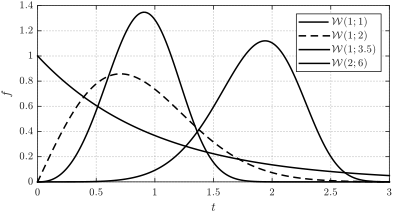
\includegraphics[width=0.9\textwidth]{plots/ma_abb2.1_weibull}
    \caption{Weibull $\sym{f}(\sym{t})$ für ausgewählte Werte von $\sym{T}$ und $\sym{b}$. }
    \label{fig:abb2.1_weibull}
\end{figure}

\subsection{Parameterschätzverfahren} \label{subsec:schätzer}
Soll eine geschlossene mathematische Beschreibung des stochastischen Ausfallverhaltens eines Produktes gefunden werden, ist das im vorherigen Abschnitten~\ref{subsec:stat} definierte parametrische Verteilungsmodell $\sym{tau} \sim \sym{W}(\sym{T}, \sym{b})$ zu schätzen.
Die Modellparameter der Grundgesamtheit sind in der praktischen Anwendung jedoch unbekannt.
Die zentrale Problemstellung der \textbf{Parameterschätzung} besteht somit darin, aus der empirischen Stichprobe bestehend aus $\sym{n}$ Realisierungen $\sym{t}_{1}, \dots, \symsub{t}{n}$ der Zufallsvariable $\sym{tau}$ statistisch fundierte Schätzwerte $\hat{\sym{T}}$ und $\hat{\sym{b}}$ zu gewinnen.
Diese sind Voraussetzung, um das Lebensdauermodell (z.B. Gleichung~\eqref{eq:weibull_cdf}) zu quantifizieren und prädiktive Aussagen zu Quantilen oder der Zuverlässigkeit $\sym{R}(\sym{t})$ zu ermöglichen.
Eine wesentliche Komplikation hierbei sind jedoch das mögliche Auftreten von unvollständigen bzw. \textbf{zensierten} Daten sowie \textit{multivariate} Abhängigkeiten der Belastungen zur Messgröße.
Während für die Schätzung von Verteilungsparametern einfache Verfahren, wie die \textbf{Momentenmethode} oder die \textbf{Methode der kleinsten Fehlerquadrate} - engl. \ac{OLS}, die beispielsweise bei der \ac{MMR} im Wahrscheinlichkeitsnetz Anwendung findet, existieren, sind diese für die umfassende Analyse vielschichtiger Lebensdauerdaten in der Regel unzureichend und hier nur der Vollständigkeit wegen erwähnt - vgl. \cite{Bertsche.2022,Montgomery.2021}.
Das universell anwendbare und robuste Verfahren, das Herausforderungen wie zensierte Daten und multivariate Modelle inhärent behandelt, ist die \ac{MLE} \cite{Meeker.2022,Nelson.1990}.

\subsubsection{Maximum-Likelihood-Estimation} \label{subsubsec:mle}
Das Grundprinzip der \ac{MLE} besteht darin, diejenigen Parameterwerte (z.B. $\hat{\sym{T}}, \hat{\sym{b}}$) als Schätzwerte auszuwählen, welche die Wahrscheinlichkeit (engl. Likelihood) maximieren, die empirisch beobachtete Stichprobe (bestehend aus unabhängigen Ausfällen und Zensierungen) zu erhalten.
Mathematisch wird die Wahrscheinlichkeit der Realisierung von $\sym{t_vec} = (\sym{t}_{1}, \dots, \symsub{t}{n})$ einer Stichprobe durch die \textbf{Likelihood-Funktion} $\sym{L_like}$ bestimmt. Diese ist eine Funktion des unbekannten Parametervektors $\sym{theta}$, der $\sym{k}$ zu schätzende Parameter enthält (z.B. $\sym{theta} = (\sym{T}, \sym{b})$ mit $\sym{k}=2$).\

Für den vereinfachten Fall, dass die Stichprobe ausschließlich aus $\sym{n}$ exakten Ausfallereignissen (vollständige Daten) besteht, ist die Likelihood-Funktion $\sym{L_like}$ das Produkt der einzelnen Wahrscheinlichkeitsdichten $\sym{f}(\cdot)$:
\begin{equation} \label{eq:mle_likelihood_simple}
    \sym{L_like}(\sym{t_vec} | \sym{theta}) = \prod_{\sym{i}=1}^{\sym{n}} \sym{f}(\symsub{t}{i} | \sym{theta}).
\end{equation}
Zur Vereinfachung der numerischen Berechnung wird in der Anwendung die \textbf{Log-Likelihood-Funktion} $\sym{Lambda}$ verwendet. Durch die Logarithmierung wird das Produkt (Gleichung~\eqref{eq:mle_likelihood_simple}) in eine äquivalente, leichter zu maximierende Summe überführt:
\begin{equation} \label{eq:mle_loglikelihood_simple}
    \sym{Lambda} \defeq \ln\left( \sym{L_like}(\sym{theta}) \right) = \sum_{\sym{i}=1}^{\sym{n}} \ln \left[ \sym{f}(\symsub{t}{i} | \sym{theta}) \right].
\end{equation}
Wie zuvor dargelegt, ist dieser vereinfachte Ansatz für Lebensdauerdaten jedoch oft unzureichend, da er das Auftreten von zensierten Daten vernachlässigt.
Für die praktische Anwendung existiert jedoch die entsprechende Erweiterung der Likelihood-Funktion um die Differenzierung etwaiger Testausgänge als \textit{Durchläufer}.
Dazu wird die Stichprobe als Paarung von $\symsub{t}{i}, \symsub{delta}{i}$ für $\sym{t_vec}$ definiert, wobei $\symsub{t}{i}$ der beobachteten Zeit und $\symsub{delta}{i}$ einem Statusindikator ($\symsub{delta}{i}=1$ für einen exakten Ausfall; $\symsub{delta}{i}=0$ für eine Rechts-Zensierung) entspricht \cite{Meeker.2022,Kalbfleisch.2002}.
$\sym{L_like}$ für rechts-zensierte Lebensdauerdaten lautet somit:
\begin{equation} \label{eq:mle_likelihood_censored}
    \sym{L_like}(\sym{t_vec} | \sym{theta}) = \prod_{\sym{i}=1}^{\sym{n}} \left[ \sym{f}(\symsub{t}{i} | \sym{theta})^{\symsub{delta}{i}} \cdot \sym{R}(\symsub{t}{i} | \sym{theta})^{1 - \symsub{delta}{i}} \right]
\end{equation}
und definiert die Log-Likelihood Funktion als:
\begin{equation} \label{eq:mle_loglikelihood_censored}
    \sym{Lambda} \defeq \ln\left(\sym{L_like}(\sym{t_vec} | \sym{theta})\right) = \sum_{\sym{i}=1}^{\sym{n}} \left[ \symsub{delta}{i} \cdot \ln \sym{f}(\symsub{t}{i} | \sym{theta}) + (1 - \symsub{delta}{i}) \cdot \ln \sym{R}(\symsub{t}{i} | \sym{theta}) \right].
\end{equation}

Der Parametervektor $\hat{\sym{theta}}$, der den Wert von $\sym{Lambda}(\sym{theta})$ maximiert, liefert die \ac{MLE}-Werte.
Die Schätzwerte repräsentieren die (asymptotisch) effizientesten Schätzwerte für die Parameter der Grundgesamtheit.
Dies erfolgt mathematisch durch Nullsetzen $\sym{k}$ partieller Ableitungen von $\sym{Lambda}$, sofern mathematisch entsprechende Schätzwerte in geschlossener Form durch $\partial\sym{Lambda}/\partial \sym{theta} \stackrel{!}{=} 0$ identifiziert werden können \cite{Nelson.2005,Rinne.2008}.
Andernfalls werden numerische Optimierungsalgorithmen, vgl. Newton-Raphson-Verfahren, Patternsearch und vergleichbare, dafür herangezogen - siehe weiterführend \cite{Nelson.2005,Qiao.1994} sowie detaillierte Untersuchungen von \textcite{Kremer.2019b}.
An dieser Stelle sei erwähnt, dass systematische Verzerrungen (engl. \textbf{Bias}) in $\hat{\sym{theta}}$ aufgrund kleiner Stichprobenumfänge auftreten können \cite{Abernethy.2006} - jedoch auch korrigierbar sind, vgl. Arbeiten von \textcite{Hirose.1999,Ross.1996}.

Die Qualität der Parameterschätzung beeinflusst daraus nicht nur die Prädiktionsgüte zur Schätzung der Lebensdauer oder Zuverlässigkeit - sie bedingt schließlich auch die Effizienz des Schätzverfahrens.
Wird im Sinne eines effizienten Verfahrens zur multivariaten Lebensdauermodellbildung eine Methodik gesucht, ist auch die Qualität der Parameterschätzung damit entscheidend.
Vertrauensbereiche, oder engl. \acp{CI}, können eine Metrik für die Qualität der Modellierung einnehmen, da sie die Unsicherheit oder \textit{Unschärfe} in der Prädiktion bemessen.


\subsubsection{Vertrauensbereiche} \label{subsubsec:ci}
Die \ac{MLE} liefert nicht nur die Punktschätzer $\hat{\sym{theta}}$, sondern auch die Quantifizierung von deren statistischer Unsicherheit (Präzision).
Obwohl verschiedene Ansätze, wie die numerisch anspruchsvolleren Berechnungen nach Likelihood-Ratio-Methode, Bootstrap-Perzentil-Methode oder Monte-Carlo-Approximation existieren, ist das gängigste Verfahren zur Berechnung von \acp{CI} die Approximation mittels asymptotischer Normalverteilung der \ac{MLE}-Schätzer $\hat{\sym{theta}}$ \cite{Bertsche.2022,Nelson.1990}.
Dies erfolgt über die \textbf{Fisher-Informationsmatrix} $\sym{FIM}$, welche die Information der Stichprobe über die Parameter $\sym{theta}$ gemäß \textcite{Kremer.2019c}  bezüglich des Rechenaufwands und resultierender Modellqualität vergleichsweise effizient quantifiziert.
So wird diese Methodik auch in gängiger Applikationen als Standard angewandt, vgl. \cite{Nelson.2005,Nelson.1990,Yang.2007}.
In der praktischen Anwendung wird die Fisher-Informationsmatrix auf Basis der resultierenden Schätzwerte $\hat{\sym{theta}} = \sym{theta}$ so als Schätzung zur Beobachtung nach $\symsub{FIM}{O}$ verwendet \cite{Nelson.1990,Lawless.2003}.
Diese ist definiert als die negative \textbf{Hesse-Matrix} $\sym{H}$ der Log-Likelihood-Funktion, ausgewertet an der Stelle der \ac{MLE}-Schätzwerte
$\hat{\sym{theta}}$:
\begin{equation} \label{eq:fim_o}
    \symsub{FIM}{O} \defeq - \sym{H}(\hat{\sym{theta}}) = - \left[ \frac{\partial^2 \sym{Lambda}(\sym{theta})}{\partial \symsub{theta}{j} \partial \symsub{theta}{l}} \right]_{\sym{theta} = \hat{\sym{theta}}}.
\end{equation}
Die Matrix $\sym{H}$ entspricht der ($\sym{k} \times \sym{k}$)-Matrix der $\sym{k}$ zweiten partiellen Ableitungen von $\sym{Lambda}$ (vgl. Gl.~\eqref{eq:mle_loglikelihood_censored}).
Eine Invertierung ${\hat{\sym{FIM}}_{\sym{O}}}^{-1}$ ergibt die geschätzte \textbf{Varianz-Kovarianz-Matrix} $\hat{\sym{V}}$:
\begin{equation} \label{eq:var_covar}
    \hat{\sym{V}} \approx {\hat{\sym{FIM}}_{\sym{O}}}^{-1}.
\end{equation}
Die Diagonalelemente dieser Matrix $\hat{\sym{V}}_{\sym{j}\sym{j}}$ entsprechen den Varianzen $\sym{Var}(\hat{\sym{theta}}_{\sym{j}})$ der einzelnen Parameterschätzwerte \cite{Nelson.1990}.
Die Nicht-Diagonalelemente $\hat{\sym{V}}_{\sym{j}\sym{l}}$ (für $\sym{j} \neq \sym{l}$) repräsentieren die \textbf{Kovarianzen} $\sym{Cov}(\hat{\sym{theta}}_{\sym{j}}, \hat{\sym{theta}}_{\sym{l}})$ \cite{Nelson.1990,Yang.2007}.
Diese Kovarianzen sind von entscheidender Bedeutung, da sie die statistische Abhängigkeit zwischen den Schätzwerten (z.B. zwischen $\hat{\sym{T}}$ und $\hat{\sym{b}}$) quantifizieren, welche für die Berechnung der \acp{CI} von abgeleiteten Funktionen wie $\hat{\sym{R}}(\sym{t})$ erforderlich sind \cite{Meeker.2022}.
Basierend auf der Annahme der asymptotischen Normalität der Schätzer wird ein zweiseitiges $(1-\sym{alpha})$-\ac{CI} für einen einzelnen Parameter $\hat{\sym{theta}}_{\sym{j}}$ direkt aus dessen Varianz approximiert durch:
\begin{equation} \label{eq:ci_normal}
    [\sym{theta}_{\sym{j},\sym{u}},\sym{theta}_{\sym{j},\sym{o}}]  = \hat{\sym{theta}}_{\sym{j}} \pm \sym{z}_{1-\sym{alpha}/2} \cdot \sqrt{\hat{\sym{V}}_{\sym{j}\sym{j}}},
\end{equation}
wobei $\sym{z}_{1-\sym{alpha}/2}$ dem $(1-\sym{alpha}/2)$-Quantil der Standardnormalverteilung entspricht.
Da Lebensdauerparameter (z.B. $\sym{T}, \sym{b}$) oft auf $\sym{RR}_{>0}$ beschränkt sind, werden \acp{CI} robust über eine Log-Transformation der Parameter berechnet, um physikalisch unmögliche (negative) Intervallgrenzen zu vermeiden \cite{Meeker.2022,Yang.2007,Nelson.1990}:
\begin{equation} \label{eq:ci_ln}
    [\sym{theta}_{\sym{j},\sym{u}}, \sym{theta}_{\sym{j},\sym{o}}] = \hat{\sym{theta}}_{\sym{j}} \exp \left( \pm \sym{z}_{1-\sym{alpha}/2} \cdot \frac{\sqrt{\hat{\sym{V}}_{\sym{j}\sym{j}}}}{\hat{\sym{theta}}_{\sym{j}}} \right).
\end{equation}

Die Berechnung dieser \acp{CI} für Schätzwerte $\sym{g_func}(\hat{\sym{theta}})$ zu Größen wie $\hat{\sym{R}}(\sym{t})$ oder $\hat{\sym{t}}_{\sym{q}}$  erfolgt mittels \textbf{Delta-Methode} \cite{Nelson.1990,Meeker.2022}.
Dieses auf einer Taylor-Reihenentwicklung basierende Verfahren (Gauß'sche Fehlerfortpflanzung) approximiert die Varianz der Funktion $\hat{\sym{g_func}}=\sym{g_func}(\hat{\sym{theta}})$ unter Einbeziehung der gesamten Varianz-Kovarianz-Matrix.
Dazu wird der \textbf{Gradientenvektor} $\sym{g_grad}$ der Funktion $\sym{g_func}$ (z.B. $\sym{g_func} = \sym{R}(\sym{t})$) bezüglich des $\sym{k}$-dimensionalen Parametervektors $\sym{theta}$ gebildet:
\begin{equation} \label{eq:delta_method_gradient}
    \sym{g_grad} \defeq \left[ \frac{\partial \sym{g_func}(\sym{theta})}{\partial \sym{theta}_{1}}, \dots, \frac{\partial \sym{g_func}(\sym{theta})}{\partial \symsub{theta}{k}} \right]^T_{\sym{theta} = \hat{\sym{theta}}}.
\end{equation}
Die approximierte Varianz $\sym{Var}(\hat{\sym{g_func}})$ der Funktion ergibt sich dann aus:
\begin{equation} \label{eq:delta_method_variance}
    \sym{Var}(\hat{\sym{g_func}}) \approx \sym{g_grad}^T \hat{\sym{V}} \sym{g_grad}.
\end{equation}
Das Vertrauensintervall für die Funktion $\hat{\sym{g_func}}$ wird anschließend unter Verwendung dieser Varianz (bzw. des Standardfehlers $\sqrt{\sym{Var}(\hat{\sym{g_func}})}$) analog zu Gleichung~\eqref{eq:ci_normal} berechnet \cite{Bain.2017b,Yang.2007,Nelson.1990}:
\begin{equation} \label{eq:ci_rel}
    [\sym{g_func}_{\sym{u}},\sym{g_func}_{\sym{o}}]  = \hat{\sym{g_func}} \pm \sym{z}_{1-\sym{alpha}/2} \sqrt{\sym{Var}(\hat{\sym{g_func}})}.
\end{equation}
Sollen auch hier nur positive Werte für $\sym{g_func}$ berücksichtigt werden, kann eine Logarithmierung in der Berechnung der Vertrauensbereiche analog zu Gl.~\ref{eq:ci_ln} erfolgen \cite{Yang.2007}.


\section{Statistische Versuchsplanung und Modellbildung} \label{sec:doe}
Multivariate Lebensdauertests erfordern definitionsgemäß die Betrachtung mehrere $\sym{k}\geq 2$ Einflussfaktoren als Versuchsparameter.
Dementsprechend entscheidend ist das Verständnis der wesentlichen Grundlagen im Umgang mit statistischer Versuchsplanung (\ac{DoE}) für Lebensdauerdaten - auch \ac{L-DoE} genannt - sowie darauffolgend der Lebensdauermodellbildung.
Der primäre Anspruch von \ac{DoE} besteht in der effizienten Planung empirischer Datenerhebungen, um Zielgrößen in Abhängigkeit erklärender Variablen robust zu optimieren.
Dieses Paradigma lässt sich gemäß \ac{DfR} unmittelbar auf die Analyse von Lebensdauer und Zuverlässigkeit übertragen \cite{Yang.2007,Wu.2021}.
Da das globale Optimum der Zuverlässigkeitsfunktion a priori meist unbekannt ist, erfordert dessen Identifikation eine systematische Exploration eines Parameterraumes.
Eine besondere Herausforderung stellt hierbei die Integration von \ac{ALT} dar: Die Diskrepanz zwischen dem hochbelasteten Testraum (engl. Design Space) und dem regulären Prädiktionsraum (engl. Use Space oder Field Level) kann daher eine Extrapolation erzwingen, welche die Anforderungen an die Daten- und somit auch Designqualität deutlich verschärft.
Da die geometrische Struktur des Versuchsplans die erreichbare Modellierungsqualität deterministisch begrenzt, ist eine a priori Bewertung der Plangüte hier wiederum unerlässlich.
Hierfür dienen objektive Performance-Indikatoren sowie mathematische Optimalitätskriterien, vgl. \cite{Montgomery.2020,Goos.2011}.

Aufgrund dessen beschäftigt sich der Inhalt dieses Abschnitts mit einer nur gezielten Auswahl an Grundbegriffen und Metriken für multivariate Testpläne im Zusammenhang mit Lebensdauerdaten sowie vielmehr mit einer Übersicht der für Lebensdauertests geeigneten Versuchspläne und dessen Features, bevor abschließend die statistische Modellbildung beleuchtet wird.

Für eine grundsätzlichere Auseinandersetzung zu vorgeschalteten, konventionellen Methoden und Werkzeugen bezüglich \ac{DoE} sei mit Blick auf den Fokus und möglichen Umfang der vorliegenden Arbeit damit auf einschlägige Literatur von \textcite{Kleppmann.2016}, \textcite{Siebertz.2017}, \textcite{Hinkelmann.2012} sowie vornehmlich \textcite{Montgomery.2020} und \textcite{Myers.2016} verwiesen.
Diese behandeln intensiv die Inhalte konventioneller statistischer Versuchsplanung, welche um Perspektiven zu \ac{L-DoE} bereits durch am \ac{IMA} entstandenen Dissertationen von \textcite{Dazer.2019}, \textcite{Herzig.2021}, \textcite{Kremer.2021} und \textcite{Grundler.2024} fortschreitend ergänzt wird - um nur eine Auswahl relevanter Referenzen zu nennen.
Konsequenterweise wird der Umgang mit normalverteilten Daten im Rahmen des \ac{DoE}, mit Regressionsmodellierung auf Basis der \ac{ANOVA}, mit konventionellen Hypothesentests und deren Hintergründe sowie mit fundamentalen Ausführungen zu \ac{ALT} innerhalb der nachfolgenden Ausführungen nicht explizit herausgestellt.

\subsection{Grundlagen zur statistischen Versuchsplanung} \label{subsec:begriffedoe}
Die Anwendung von \ac{DoE} versteht sich grundsätzlich als Verfahrenskette \cite{Coleman.1993,Montgomery.2020} entlang mehrere Prozessschritte, die ausgehend von einer spezifischen Aufgabendefinition beginnt und in einer statistischen abgesicherten Datenmodellierung mündet, vgl. \colorbox{yellow}{Abbildung~Doe-Steps}.
Das erklärte Ziel ist es also, den kausalen Zusammenhang zwischen Einflussfaktoren und Systemantwort funktional abzubilden.
So kann dieser Zusammenhang - beispielhaft die zufallsverteilte Lebensdauer $\sym{tau}$ in Abhängigkeit $k>2$ technischer Beanspruchungen - modelliert und optimiert werden, vergleiche \textit{Schritt~1} in \colorbox{yellow}{Abbildung~Doe-Steps}.

Im Zentrum der Betrachtung steht dabei das technische \textbf{System}, welches abstrakt als Produkt oder Prozess verstanden wird und den Zustand der Ausgangsgröße in Abhängigkeit der Eingangsgrößen definiert.
Die zu untersuchende oder zu optimierende Ausgangsgröße wird generell als \textbf{Systemantwort} $\sym{y}$ (engl. Response) bezeichnet.
Die gezielt kontrollierbaren und variierten Eingangsgrößen sind die \textbf{Faktoren} (\textbf{Steuergrößen}), während nicht kontrollierbare oder unbekannte Einflüsse als \textbf{Störgrößen} (engl. Noise) klassifiziert werden, vergleiche \textit{Schritt~2} in \colorbox{yellow}{Abbildung Doe-Steps} \cite{Kleppmann.2016}.
Um ein Systemverhalten perspektivisch zu charakterisieren, werden die Faktoren als kategoriale oder kontinuierliche Parameter im Versuch auf diskreten Werten, den sogenannten \textbf{Faktorstufen} (engl. Level), variiert (\textit{Schritt~3}).
Die planerische Kombination verschiedener Faktorstufen äußert sich dann in spezifischen \textbf{Versuchspunkten} innerhalb des \textbf{Parameterraums} bzw. Design Spaces.
Anteilig erstreckt sich hierin das Volumen über die Parameterwerte, welche im Versuchs eingestellt werden können, über den \textbf{Versuchsraum} (engl. Design Space)
Statistische Versuchspläne (\textit{Schritt~4}) für die Durchführung (\textit{Schritt~5}) können nachfolgend aus Abschnitt~\ref{subsec:pläne} entnommen werden.
Die aus dieser Variation resultierende Änderung der Systemantwort quantifiziert den Einfluss des Faktors, der statistisch als \textbf{Effekt} bezeichnet und quantifiziert wird (\textit{Schritte~6-7}).
Eine visuelle Aufstellung des genannten Zusammenspiels der Parameter kann dem Paramterdiagram, kurz \textbf{P-Diagramm}, in \colorbox{yellow}{Abbildung~P-Diagram} entnommen werden.
Die hierbei erreichte Akquisition einer empirischen Datengrundlage folgt also entlang eines präzise beschriebenen Prozesses und innerhalb der Vorgaben vorab definierter Versuchspläne.
Dies ergibt entscheidende Vorteile, wird der planerische Aspekt in die Ausführung aufgenommen.
Entgegen in der Praxis üblicherweise noch verbreiteter alternativer Vorgehen wie \ac{OFAT}-Testing können mittels \ac{L-DoE} strukturiert, effizient und verbindlich Informationen gewonnen werden, die über die faktorbedingten Effekte hinaus gehen und differenziert Aufschluss über \textbf{Haupteffekte} und etwaige \textbf{Wechselwirkungen} der Faktoren geben können, vgl. \cite{Montgomery.2020,Kleppmann.2016,Siebertz.2017}.
Beide können gemäß beliebiger Polynomfunktionen höhere Ordnungen annehmen, smoit \textbf{quadratische Effekte} oder \textbf{Mehrfachwechselwirkungen} abbilden.



\subsection{Statistische Lebensdauer-Versuchspläne} \label{subsec:pläne}

\subsection{Statistische Modellbildung} \label{subsec:model}

\begin{itemize}
    \item \colorbox{yellow}{wu}
    \item \colorbox{yellow}{wütherich}
    \item \colorbox{yellow}{yang p282 erster abschnitt}
    \item \colorbox{yellow}{russell doe for glm kap1.4 p12}
\end{itemize}
\cite{RisbergEllekjr.1998, Bisgaard.1992,Bisgaard.2011,Myers.2016,Montgomery.2020,Zahran.2003,GiovannittiJensen.1989,Goos.2011,Hinkelmann.2012,Khuri.2006,Rittmaier.2025,Johnson.2011,Donev.2004,G.E.P.Box.1951,Ardakani.2011,Jones.2012,Jones.2021,Rigdon.2022,Wu.2021,Khuri.2006,Escobar.1995,Modarres.2017,Ahn.2015,Rasch.2018,Xu.2002,Wald.1943,Rencher.2008,Box.2007,Kleppmann.2016,Siebertz.2017,Fisher.1935,Bisgaard.1997,Myers.2010}